\documentclass[bachelor]{thesis-uestc}

\title{基于语法树的文档级关系预测算法设计与验证}{Design and Verification of Document-level Relation Extraction Algorithm Based on Syntax Tree}
\author{朱旭东}{Xudong Zhu}
\advisor{康昭\chinesespace 副教授}{Dr. Zhao Kang}
\school{计算机科学与工程学院(网络空间安全学院)}{School of Computer Science and Engineering}
\major{计算机科学与技术}{Computer Science and Technology}
\studentnumber{2020080902004}

\usepackage{graphicx} % for graph
\usepackage{verbatim} % multi-line comment

\begin{document}

\makecover

\begin{chineseabstract}
    文档级关系抽取旨在识别单个文档中实体对之间的关系。
    它需要处理多个句子并对这些句子进行推理。
    最先进的文档级关系抽取使用图形结构来连接文档中的实体,来捕获文档中的实体对的交互。
    但是这些方法没有充分利用在句子级关系抽取中被充分研究的语法信息。
    在本文中我们以将语法树融合到文档级关系抽取中为主要研究内容,重点研究了使用依赖语法树,依存语法树进行文档级关系抽取算法的实现,以及怎么调整依赖语法树和依存语法树的在文档级关系抽取中的权重问题。
    我们利用依存语法树来聚合整个句子信息,并为目标实体对选择有指导意义的句子。
    同时我们利用依赖语法树对整个文档进行细粒度的分析,并选择其中重要的单词增强目标实体对的信息。
    文档级关系抽取将同时利用依赖语法树和依存语法树进行预测。
    通过在不同领域的数据集上的实验结果证明了该方法的有效性。


    \chinesekeyword{文档级关系抽取,依赖语法树,依存语法树,信息抽取}
\end{chineseabstract}

\begin{englishabstract}
    Document-level Relation Extraction (DocRE) aims to identify relation labels between entity pairs within a single document.
    It requires handling several sentences and reasoning over them.
    State-of-the-art DocRE methods use a graph structure to connect entities across the document to capture interaction between entity pairs in the document.
    However, this is insufficient to fully exploit the rich syntax information in the document, which is widely used in sentence-level Relation Extraction(RE).
    In this thesis, we focus on integrating syntax trees into DocRE as the main research topic, and investigate the effective and effient implementation of DocRE algorithms using dependency syntax tree and constituency syntax tree, as well as how to adjust the weight of dependency syntax tree and constituency syntax tree in the extraction.
    It uses constituency syntax to aggregate the whole sentence information and select the instructive sentences for the pairs of targets.
    Meanwhile, it exploits the dependency syntax in a graph structure with constituency syntax enhancement and selects the most important words between entity pairs based on the dependency graph to enhance the information of target entity pairs.
    Finally, DocRE will integrate the dependency syntax and constituency syntax to predict.
    The experimental results on datasets from various domains demonstrate the effectiveness of the proposed method.


    \englishkeyword{Document-level Relation Extraction, Constituency Syntax, Dependency Syntax, Information Extraction}
\end{englishabstract}

\thesistableofcontents

\chapter{绪\hspace{6pt}论}

\section{研究的背景}
\begin{comment}
    课题背景,研究现状, 理论依据,实验基础,发展趋势以及本课题的理论意义
\end{comment}

% 两页

% 关系抽取介绍,包括背景和最近从句子级转移到文档级关系抽取
关系提取是信息提取中的一项关键任务,旨在对非结构化文本中实体对之间的关系模式进行建模。
它有两种特定的场景:句子级关系提取和文档级关系提取。
与句子级关系提取 \cite{sentenceRE-Dixit, sentenceRE-Lyu} 不同,文档级关系提取涉及识别和提取句子边界以外的实体之间的关系,为分析提供了更广泛的上下文,并且更具挑战性。
这项任务可以从非结构化的大型文档(如科学论文、法律合同或新闻文章) \cite{delaunay2023comprehensive} 中自动构建和填充知识库,以更好地理解实体之间的关系。
因此,文档级关系提取更好地满足了实际需求,最近受到了越来越多的关注。\par

% 现在关系抽取的主要方法和存在的一些缺陷

文档级关系抽取的目标是识别在同一文档内的实体对之间的关系。
这是一项复杂的任务,因为它需要理解句子的内容并处理多个句子之间的交互。
由于文档级关系抽取涉及多个句子,现在的研究有三个主要障碍 \cite{9098945}:
\begin{enumerate}
    \item \em{数量更多的潜在关系}: 相比于单个句子,一个文档中包含的实体数量更多。
    由于我们需要预测每两个实体之间的关系,因此潜在的待预测关系随着实体的增加呈指数级别增加。
    \item \em{处理实体共指}: 一个实体通常在一个句子中只出现一次,而在一个文档中,它可以以多种形式出现多次。例如,在图3的句子2和句子3中,"He"是"Marcus Miller"的共同指称。
    \item \em{处理长距离关系}: 在文档级关系抽取中,我们通常需要预测跨句子之间的关系,这可能会导致实体对之间距离过长。
    然而,长句中通常包含不相关甚至有噪声的信息。Huang等人\cite{huang-etal-2021-three} 认为,在大多数情况下,最多只需要三个句子作为识别关系的支持证据。此外,这项工作指出,句子之间的重要性差异很大。不包含任何有价值的信息或关系的句子实际上阻碍了文档的理解。这也是我们这篇论文要解决的主要工作。
\end{enumerate}
\begin{figure}[h]
    \centering
    \caption{文档级关系抽取的一个例子。图片上方是文档内容,文档中实体用不同的颜色标注,下方是文档级关系抽取的结果。}
    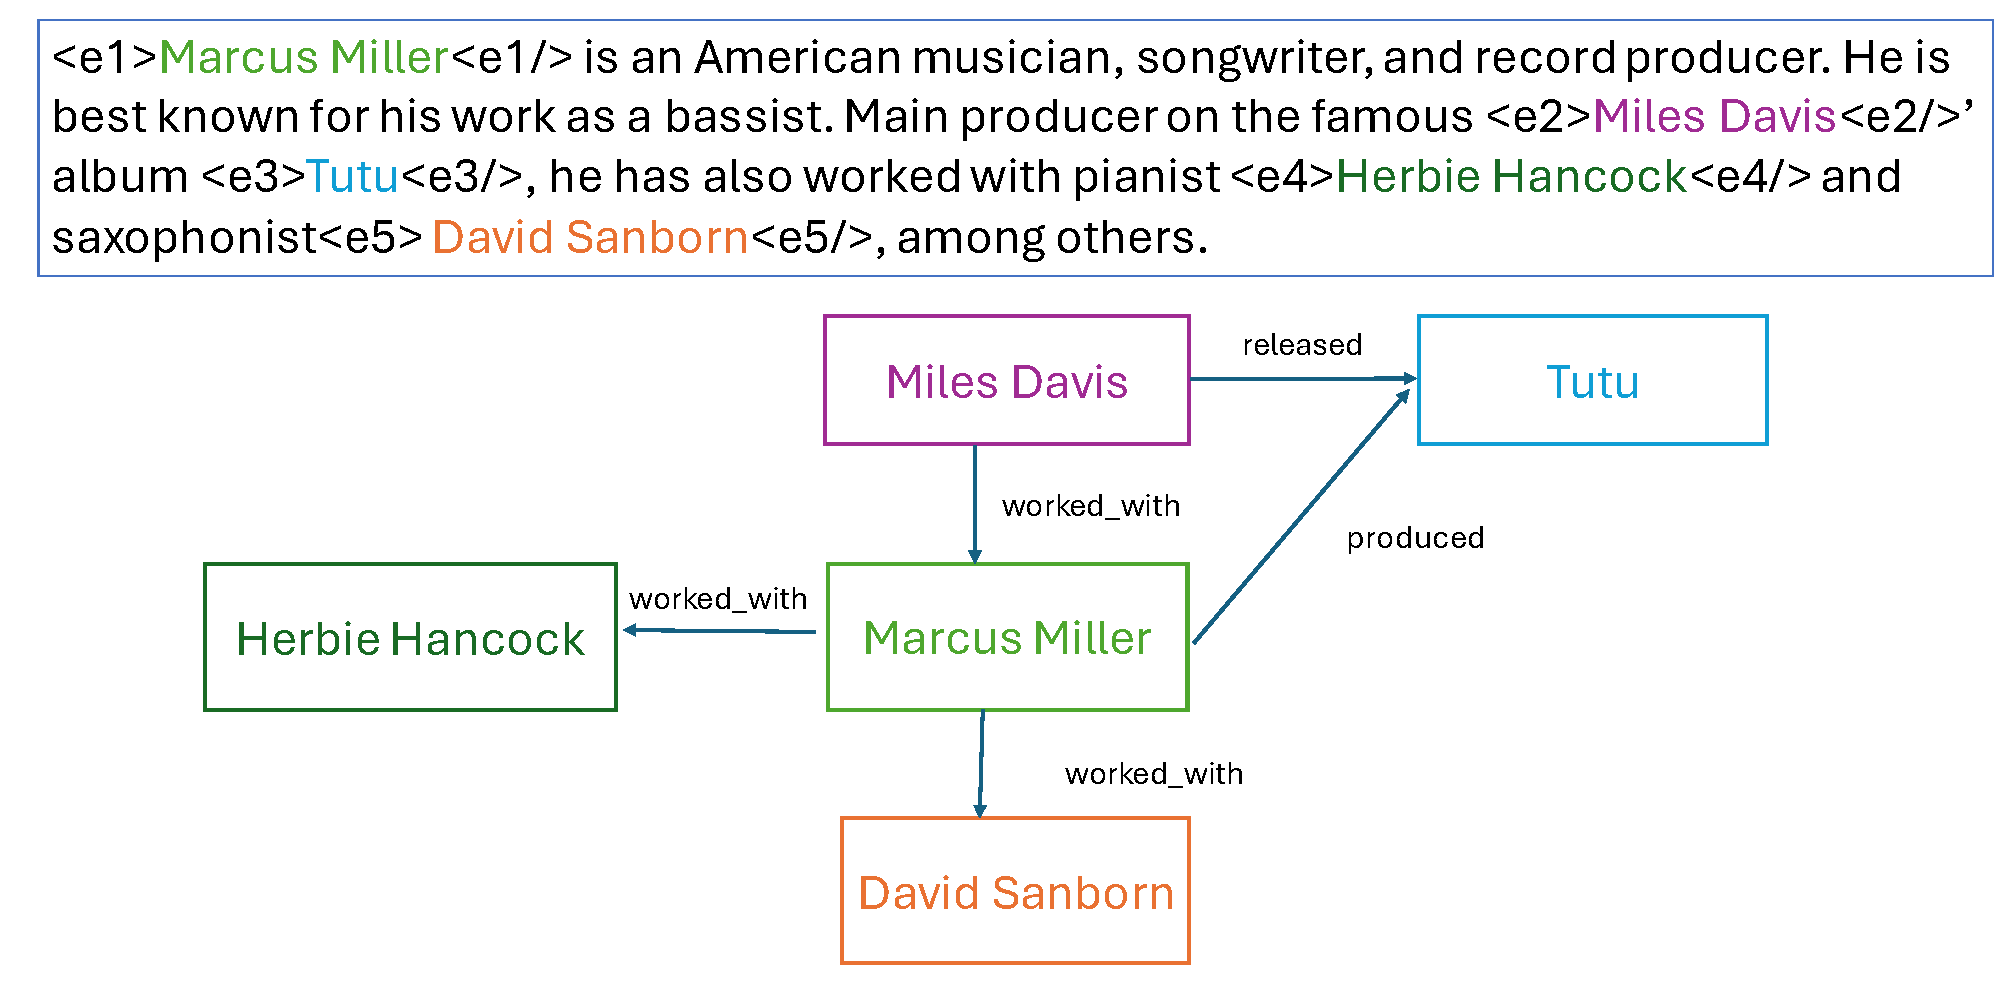
\includegraphics[width=0.8\textwidth]{misc/fig_example.pdf}
\end{figure}\label{fig_example}

图 \ref{fig_example}是一个例子,它包括来自同一文档中的句子级关系和文档级关系。
为了推断"Marcus Miller"和"Herbie Hancock"之间的关系,模型应该能够排除不相关实体的影响,并找出句子3中的"he"一词指的是"Marcus Miller"。
然而,由于现有的文档级关系提取模型 \cite{bai-etal-2021-syntax} 经常会被大量不相关的信息所淹没,从而无法捕捉到类似的关键信息。 \par

由于以上这些原因,本文提出了新的一种文档级关系提取方法,通过融合语法信息作为辅助,来改进文档级关系提取。\par

\section{研究的主要贡献与创新}
% 语法方法是如何帮助文档级关系抽取的,我们的方法大体是怎么做的
本文主要处理文档级关系提取的长距离关系。
由于长句中通常包含无关甚至嘈杂的信息 \cite{gupta2019neural},对于文档级关系提取来说,隐含地学习指导性上下文是不够的 \cite{bai-etal-2021-syntax}。
最近的一些文章通过预训练模型和注意力机制来学习文档中复杂的交互 \cite{huang-etal-2021-three, y2020-coreferential, zhou2021document}, 他们通过创建更复杂、更强大的变体transformer来隐含的捕获实体之间复杂的互动。
但是,更多的方法通过显示捕获实体互动信息来改善文档级关系抽取。他们首先构建由不同节点组成的文档图 (例如实体的提及节点,实体节点,句子节点或者文档节点) \cite{GAIN, liu2023document},将指导性上下文转化为图。
由于语法信息可以通过提供显式语法细化和子内容建模来帮助文档级关系抽取 \cite{duan-etal-2022-just},最近的研究 \cite{sahu2019inter, SagDRE} 采用依赖图来合并语法信息和结构上下文。
他们发现一个精心设计的图形可以帮助模型更好的捕获实体互动信息,缩短实体之间的距离。
然而,正如 \cite{sundararaman2019syntax, bai-etal-2021-syntax}所指出的,尽管预训练模型是用大量真实世界的文本数据进行训练的,但隐式学习的语法与黄金语法之间仍然存在很大差距。
事实上,语法信息在句子级关系抽取中得到了广泛的应用\cite{xu-etal-2016-improved, qin-etal-2021-relation},但在文档级关系抽取场景下尚未得到充分的探索。\par

为了充分利用文档中的语法信息,本文融合了依存语法和依赖语法。
我们主要采用依赖图和依存树来合并额外的语法信息,并使用依存树中的信息来进一步增强依赖图的表示。
依赖语法描述了一个句子中单词之间的依赖关系,这些依赖关系对原始纯文本有很强的补充作用。
而依存语法可以分层合理地组织单个句子的不同单词,消除了枚举不同单词组合的过程,同时保持了分层语法信息。
在树形深度学习模块 \cite{duan-etal-2022-just} 的帮助下,我们可以收集具有适当权重的所有子内容,以解决句间依赖关系并融合依赖语法产生最终关系预测。\par

% 总结,我们的贡献

通过对三个公共文档级关系抽取数据集 (DocRED \cite{DOCRED}、CDR \cite{li2016biocreative} 和GDA \cite{GDA} )的广泛实验下,我们证明我们的算法在很大程度上优于现有方法。
我们在这篇文章中的主要贡献可以总结如下:
\begin{enumerate}
    \item 我们建议利用依存语法树来聚合句子级信息,以弥补依赖语法树中的差距,并通过添加文档节点来改进依赖图,以减少实体对的距离,简化长句交互。
    \item 我们分别用Tree-LSTM和GCN处理转化后的依赖语法和依存语法,并设置一个可学习的参数来调整它们的权重。
    \item 实验结果表明,我们的模型在三个公共文档级关系抽取数据集上的测试优于现有方法,特别是在DocRED上,我们的模型将最先进方法的IgnF1提高了至少1.56\%
\end{enumerate}

\section{研究的结构安排}
本研究的后续方式组织: 第二章主要介绍文档级关系抽取的研究现状,在这一章中,我们对过往的研究结果进行总结。第三章介绍我们的研究工作,包括我们依赖语法和依存语法的使用方式,以及如何调节这两种语法的权重。第四章报告了我们研究的实验结果,包括在三个公共文档级关系抽取数据集上的不同指标的分数,与过往研究的分数对比以及分析;同时包括了对我们方法的每个模块的分析。
\begin{comment}
    课题的方案论证,包括课题的主要任务,功能要求,性能指标等
    课题的工作
    A. 理论课题
(a) 理论基础和原理
(b) 理论分析、推导、数学模型
(c) 模型仿真(含数据、曲线等)

also: 图表的标注先写在图表的上方,明天再次询问这个问题
\end{comment}
\chapter{关系抽取研究}
在这一部分,我们首先对关系抽取进行定义。
然后我们介绍对文档级关系方法的回顾。
\section{关系抽取的定义}
% 一页

在这篇文章中,我们遵循Zhang等人提出的定义 \cite{zhang-etal-2020-document}。
对于每个预测任务,我们有文档$D=\{S_i\}_{i=1}^{n_s}$和实体集合$E=\{e_i\}_{i=1}^{n_e}$。
其中$n_s$是文档中句子的数量,$n_e$是实体的数量,在句子级关系抽取中$n_s$被固定为1,但是在文档级关系抽取中没有限制。
文档中的句子被表示为$S_i=\{w_j\}_{j=1}^{n_w^j}$,其中$w_i$是第$i$个句子中的第$j$个单词。
每一个实体被表示为$E_i=\{m_j\}_{j=1}^{n_w^j}$,其中$m_i$是第$i$个实体中的第$j$个提及。
在句子级别设置中,一个实体只由一个提及表示,即$\forall i \in [1, n_e], e_i = m_i$, 但是在在文档级关系抽取中情况并非如此,其中实体可以通过多次提及来表示。
为了获得实体的固定表示,以前的方法首先对所有提及的嵌入进行平均,即 $e_i = \frac{\sum_{j=1}^{n_m^j} m_j}{n_m^i}$,或者对所有提及的嵌入进行最大池化。
然而,现在的方法都使用更加柔和的logsumexp表示,即 $e_i = \log \sum_{j=1}^{n_m^j} \exp(m_j)$,这样可以促进来自弱提及信息的积累 \cite{jia-etal-2019-document}。
我们也采用这种方式表示每一个实体。\par

文档级关系抽取的目标是正确推断每个实体对$(e_s,e_o)_{s,o = 1, 2, \dots, n_e}; s \neq o$之间的关系。
其中$e_s$是头实体, $e_o$是尾实体。
预测的关系是预定义的关系集合$R$或者$NA$(没有关系)的子集。

\section{文档级关系抽取}
本节介绍了文档级关系抽取的最新进展,重点介绍基于序列的,基于注意力机制的和基于语法树的文档级关系抽取方法,并分析他们的优缺点。

\subsection{基于序列的文档级关系抽取}
执行文档级关系提取的一种方法是将文档视为一个长的增强的序列,并应用从句子级关系抽取导出的序列模型来识别特定实体之间的关系。

\subsubsection{基于卷积神经网络的文档级关系抽取}
Gu等人 \cite{10.1093/database/bax024}通过两个分离的模型来提取关系。
他们首先将最大熵系统用于句子间的预测,卷积神经网络模型用于句子内的预测。
然后,这两个结果被合并以获得文档级别的关系。
此外,他们还定义了一些启发式规则来从摘要中提取关系,例如将论文标题中提到的所有化学物质(或如有必要,将摘要中最频繁的化学物质)与摘要中提及的所有疾病相关联。\par

李等人 \cite{li2018chemical}
使用递归分段卷积神经网络进行化关系提取,并结合了领域知识、分段策略、注意力机制和多实例学习。
该方法首先利用分段卷积神经网络来捕获单个实例的表示。
然后,使用递归神经网络来聚合实例的表示,从而能够为实体对形成全面的文档级表示。

\subsubsection{结合卷积神经网络和递归神经网络的文档级关系抽取}
Mandya等人 \cite{mandya2018combining}提出了一种长短期记忆和卷积神经网络的组合模型,该模型利用单词嵌入和位置嵌入来提取跨句子的$n$元关系。
长短期记忆模型将结合单词嵌入和位置特征的变换矢量表示作为输入,将输出被馈送到卷积神经网络中。
卷积神经网络被用来提取最重要的特征。
这种方法的优点是独立于复杂的句法特征,如依赖树、共指消解或话语特征。因此被广泛应用到后续的改进模型中。

为了提取基因-疾病相关性,Wu等人 \cite{wu2019renet}还在其方法中结合了门控神经单元。
在这里,卷积神经网络首先使用具有不同宽度的不同滤波器从单词表示中计算句子表示,以捕捉不同的特征。
然后,门控神经单元将它们转换为文档表示。
通过消融实验,他们发现,即使单独的卷积神经网络也可能捕捉到文档的一些重要特征,而额外的门控神经单元层可以提高其性能。
这项研究后来被Su等人 \cite{renet2} 进行了扩展。
在Wu等人的系统之前引入了部分过滤步骤,来删除不包含任何实体对信息和模糊关系的段落。

\subsubsection{以实体为中心的文档级关系抽取}
在传统的句子级关系抽取中,对提及元组进行分类预测就已经足够了,但是在文档级关系抽取中却不是这样。
因为任何实体都可能有多次提及,应用简单的提及级别分类方法会使模型在大量的提及中淹没,导致预测失败。
为了解决这个问题,Jia等人 \cite{jia-etal-2019-document} 提出通过对每个实体元组进行单一关系预测,使用以实体为中心的多尺度预测。它们通过对实体的所有上述表示应用logsumexp来获得实体表示。

\subsubsection{基于序列的文档级关系抽取总结}
这些方法通过将文档视为一个长的增强的序列,将句子级关系抽取的方法自然的映射到文档级关系抽取上。
这些方法的优点是能够处理长文档,并且能够利用跨句子的关系信息。
然而,当待预测实体对涉及到处理长距离并需要多跳推理上下文内容时,这些模型不可避免地会遇到挑战。

\subsection{基于注意力机制的文档级关系抽取}
% 三页

\subsection{基于语法树的文档级关系抽取}
% 三页
\section{本章小结}
\newpage
1

\newpage

\chapter{基于语法树的文档级关系抽取研究}
% 说明文字和方法图表, 一页

\section{基于依存语法树的文档级关系抽取}
% 两页

\section{基于依赖语法树的文档级关系抽取}
% 两页

\section{融合两种不同语法树结果的文档级关系抽取}
% 两页

\section{本章小结}
\newpage
1
\newpage


\chapter{基于语法树的文档级关系抽取实验结果}
为了全面的评估我们的模型,我们在来自不同领域的三个文档级数据集上评估了我们的算法模型。
我们在第 \ref{sec:dataset}节介绍了这些模型,在第 \ref{sec:docred}和 \ref{sec:medical}节说明了我们的结果。
然后,我们在第 \ref{sec:weight}节分析了两种不同的语法树权重,在第 \ref{sec:distance}节分析了依赖语法树路径距离。
最后,我们在第 \ref{sec:inter}节进行了消融实验,并总结了我们的研究结果。

\section{文档级关系抽取抽取数据集说明}\label{sec:dataset}

\begin{table}[h]
    \caption{三个公共数据集的统计数据}
    \begin{tabular}{cccc}
    \hline
    统计数据               & DocRED & CDR & GDA   \\ \hline
    \# 训练集                 & 3053   & 500 & 23353 \\
    \# 验证集                   & 1000   & 500 & 5839  \\
    \# 测试集                  & 1000   & 500 & 1000  \\
    \# 关系数量             & 96     & 2   & 2     \\
    \# 平均每篇文章的句子数量 & 8.0    & 9.7 & 10.2  \\ \hline
    \end{tabular}
\end{table} \label{table:datasets}

我们在三个公共数据集上评估了我们的模型,表 \ref{table:datasets}列出了这些数据集的统计数据。
\begin{itemize}
    \item \textbf{DocRED} \cite{DOCRED} 是一个从维基百科中人为标注的大型数据集。
    它包含从维基百科中采样的5053个黄金注释文档,132275个实体、56354个关系事实和96个关系类,每篇平均长度为196.7个单词,超过40.7\%的关系对是跨句关系事实。
    实体部分包括经典的实体标签,如PERSON、ORGANIZATION和LOCATION;而实体关系部分使用了96种关系类型,涵盖了广泛的科目, 包括科学(33.3\%)、艺术(11.5\%)、时间(8.3\%)、个人生活(4.2\%)等。
    \item \textbf{CDR} \cite{li2016biocreative} 是一个生物医学的文档级关系抽取数据集,由1500篇PubMed的摘要组成。
    这些摘要被随机分为三个相等的部分进行训练、验证和测试。
    这个数据集的预测任务是预测化学品和疾病之间的二元关系。
    \item \textbf{GDA} \cite{GDA} 
    也是一个生物医学的文档级关系抽取数据集,包含30192篇摘要。
    这个大型数据集是通过对公开数据库收集的基因-疾病关联中的30192篇摘要(测试集为1000篇,其余按80:20的比例在训练集和验证集之间划分)进行远程监督构建的。
    这个数据集的预测任务是预测基因和疾病之间的二元关系。
\end{itemize}

\section{DocRED数据集实验结果说明与分析}\label{sec:docred}

\section{医学数据集实验结果说明与分析}\label{sec:medical}

\section{两种不同的语法树权重分析}\label{sec:weight}

\section{依赖语法树路径距离分析}\label{sec:distance}

\section{消融实验结果说明与分析}\label{sec:inter}

\section{本章小结}\label{sec:conclusion}
\newpage
1
\newpage
\chapter{结论}
1
\begin{comment}
    在工作总结的基础上,经过分析、归纳,明确结论:
①系统功能、指标等是否实现或达到课题要求(工程技
术及软件课题)
②理论结果是否正确、所建模型是否合理(理论课题)
41③所阐述的观点是否正确(文科课题)
④本课题有待进一步解决的问题及方向
⑤本人收获及体会
\end{comment}
\thesisacknowledgement
在攻读计算机学士学位期间,首先热烈感谢我的导师康昭教授。经过风风雨雨的研究,我得到了他的无私关怀和支持。在此特别表达感谢之情。我还要感谢我的一直以来的帮助者们,包括学院的老师、同学、同事,以及所有支持和关心我的人。我也要感谢我的家人,他们给予我强大的内心支持和生活的安定和稳定。

% Uncomment to list all the entries of the database.
%\bibliography command
%\nocite{*}
%\thesisbibliography{reference}

%
% Uncomment following codes to load bibliography database with native
%\bibliography command.

\bibliographystyle{thesis-uestc}
\bibliography{reference}


%\thesistranslationoriginal
%\section{The OFDM Model of Multiple Carrier Waves}

%\thesistranslationchinese
%\section{基于多载波索引键控的正交频分多路复用系统模型}

\end{document}
